\documentclass{beamer}

\usepackage[utf8]{inputenc}

\usepackage{amsmath}
\usepackage{amsfonts}
\usepackage{amssymb}
\usepackage{amsthm}
\usepackage[ukrainian,russian]{babel}

\usepackage{fontenc}
\usepackage{graphicx}

\usepackage{tikz}

\usepackage{ulem}

\usepackage{listings}
\usepackage{color}

\usepackage{hyperref}
\usepackage{latexsym,url}
\usepackage{braket}




\usetheme{Warsaw}
\author{Ширай Андрей}
 \institute{}
\title{Квантовая информатика -- что, зачем и почему?}
\date{\today}

\newtheorem{defin}{Определение}
\newtheorem{theor}{Теорема}
\newtheorem{astat}{}
\newtheorem{stat}{Постулат}

\begin{document}
\frame{\titlepage}

\frame{
\frametitle{We have a plan!}

\begin{itemize}
 \item Исторический экскурс.
 \item Как это работает.
 \item Примеры физических реализаций.
 \item Квантовые алгоритмы Шора(факторизация) и Гровера(поиск по неупорядоченной БД).
 \item Как это повлияет на надежность криптосистем?
 \item Как квантовая информатика повлияла на другие направления теоретической 
информатики/математики/физики.
 \item Моделирование квантовых вычислений
\end{itemize}

}

% % % % % % % % % % % % % % 


\frame{
\frametitle{Вы, конечно же шутите, мистер Фейнман!}
\begin{center}
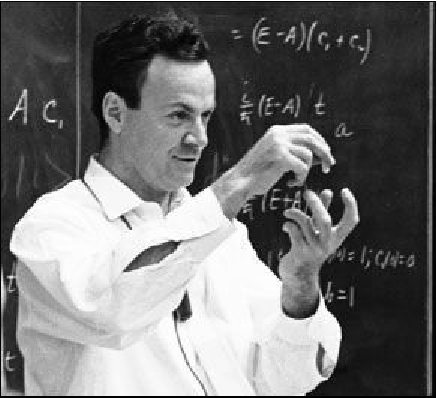
\includegraphics[scale=0.7]{f.pdf}


Feynman, R. P. (1982). \textit{"Simulating physics with computers"}. International Journal of Theoretical Physics 21 (6): 467–488. 

\end{center}


}

% % % % % % % % % % % % % % 

\frame{

\frametitle{Освой линейную алгебру за 240 секунд!}

\[
\begin{pmatrix}\frac{1}{2} & 0 \cr 0 & \frac{1}{2}\end{pmatrix}
\begin{pmatrix}1\cr 0 \end{pmatrix} =
\begin{pmatrix}\frac{1}{2}\cr 0 \end{pmatrix}
\]

\begin{center}
\begin{tabular}{ll}
\begin{tikzpicture}[scale=2]
% \clip (-4.63205,-1.88345) rectangle (4.06915,1.88345);
\draw [step=.1cm, help lines] (0,0) grid (1,1);
\draw [help lines] (-1,0) grid (0,1);
\draw [help lines] (0,-1) grid (1,0);
\draw [help lines] (-1,-1) grid (0,0);
\draw [color=black,->] (-1,0) -- (1,0);
\draw [color=black,->] (0,-1) -- (0,1);
%% вектор;
\draw[blue, line width=1pt, solid, ->] (0,0) -- (1,0);

\end{tikzpicture} & 
\begin{tikzpicture}[scale=2]
% \clip (-4.63205,-1.88345) rectangle (4.06915,1.88345);
\draw [step=.1cm,help lines] (0,0) grid (1,1);
\draw [help lines] (-1,0) grid (0,1);
\draw [help lines] (0,-1) grid (1,0);
\draw [help lines] (-1,-1) grid (0,0);
\draw [color=black,->] (-1,0) -- (1,0);
\draw [color=black,->] (0,-1) -- (0,1);
%% вектор;
\draw[blue, line width=1pt, solid, ->] (0,0) -- (0.5,0);

\end{tikzpicture} 
\end{tabular}
\end{center}

}

\frame{

\frametitle{Освой линейную алгебру за 240 секунд!}
\[
\begin{pmatrix}\frac{1}{\sqrt{2}} & \frac{1}{\sqrt{2}}\cr \frac{1}{\sqrt{2}} & -\frac{1}{\sqrt{2}}\end{pmatrix}
\begin{pmatrix}1\cr 0\end{pmatrix} =
\begin{pmatrix}\frac{1}{\sqrt{2}}\cr \frac{1}{\sqrt{2}}\end{pmatrix}
\]

\begin{center}
\begin{tabular}{ll}
\begin{tikzpicture}[scale=2]
% \clip (-4.63205,-1.88345) rectangle (4.06915,1.88345);
\draw [step=.1cm,help lines] (0,0) grid (1,1);
\draw [help lines] (-1,0) grid (0,1);
\draw [help lines] (0,-1) grid (1,0);
\draw [help lines] (-1,-1) grid (0,0);
\draw [color=black,->] (-1,0) -- (1,0);
\draw [color=black,->] (0,-1) -- (0,1);
%% вектор;
\draw[blue, line width=1pt, solid, ->] (0,0) -- (1,0);

\end{tikzpicture} & 
\begin{tikzpicture}[scale=2]
% \clip (-4.63205,-1.88345) rectangle (4.06915,1.88345);
\draw [step=.1cm,help lines] (0,0) grid (1,1);
\draw [help lines] (-1,0) grid (0,1);
\draw [help lines] (0,-1) grid (1,0);
\draw [help lines] (-1,-1) grid (0,0);
\draw [color=black,->] (-1,0) -- (1,0);
\draw [color=black,->] (0,-1) -- (0,1);
%% вектор;
\draw[blue, line width=1pt, solid, ->] (0,0) -- (0.707,0.707);

\end{tikzpicture} 
\end{tabular}
\end{center}








}


\frame{

\frametitle{Освой линейную алгебру за 240 секунд!}

\begin{defin}
 \textbf{Cобственный вектор} -- любой ненулевой вектор $\vec{x}$, который отображается оператором в коллинеарный $\lambda \vec{x}$, а соответствующий скаляр $\lambda$ называется \textit{собственным значением} оператора.
\end{defin}

\[
\begin{pmatrix}\frac{1}{\sqrt{2}} & \frac{1}{\sqrt{2}}\cr \frac{1}{\sqrt{2}} & -\frac{1}{\sqrt{2}}\end{pmatrix}
\begin{pmatrix}1\cr -\sqrt{2}-1\end{pmatrix} =
\begin{pmatrix}-1\cr \sqrt{2}+1\end{pmatrix}
\]

\begin{center}
\begin{tabular}{ll}
\begin{tikzpicture}[scale=1]
% \clip (-4.63205,-1.88345) rectangle (4.06915,1.88345);
\draw [step=.1cm,help lines] (0,0) grid (1,1);
\draw [help lines] (-1,0) grid (0,1);
\draw [help lines] (0,-1) grid (1,0);
\draw [help lines] (-1,-1) grid (0,0);
\draw [color=black,->] (-1,0) -- (1,0);
\draw [color=black,->] (0,-1) -- (0,1);
%% вектор;
\draw[blue, line width=1pt, solid, ->] (0,0) -- (1,0);
\draw[red, line width=1pt, solid, ->] (0,0) -- (1,-2.414);

\end{tikzpicture} & 
\begin{tikzpicture}[scale=1]
% \clip (-4.63205,-1.88345) rectangle (4.06915,1.88345);
\draw [step=.1cm,help lines] (0,0) grid (1,1);
\draw [help lines] (-1,0) grid (0,1);
\draw [help lines] (0,-1) grid (1,0);
\draw [help lines] (-1,-1) grid (0,0);
\draw [color=black,->] (-1,0) -- (1,0);
\draw [color=black,->] (0,-1) -- (0,1);
%% вектор;
\draw[blue, line width=1pt, solid, ->] (0,0) -- (0.707,0.707);
\draw[red, line width=1pt, solid, ->] (0,0) -- (-1,2.414);

\end{tikzpicture} 
\end{tabular}
\end{center}



}

\frame{

\frametitle{Стохастические вычисления}


\begin{center}
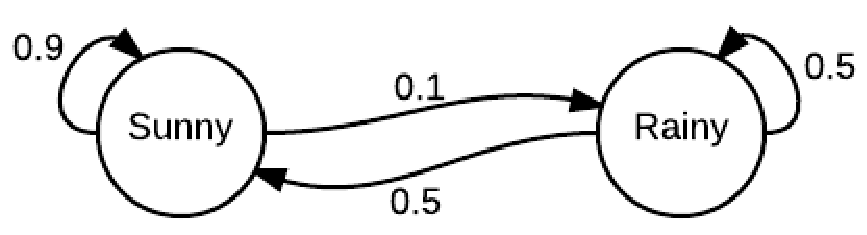
\includegraphics[scale=0.5]{mar.pdf}
\end{center}


$P= \begin{pmatrix}0.9 & 0.5\cr 0.1 & 0.5\end{pmatrix}$ --матрица перехода для некоторой цепи Маркова.
Входные данные: $x=\begin{pmatrix}1\cr 0\end{pmatrix}$ -- у нас хорошая погода.
\[
\begin{pmatrix}0.9 & 0.5\cr 0.1 & 0.5\end{pmatrix}
\begin{pmatrix}1\cr 0\end{pmatrix} =
\begin{pmatrix}0.9\cr 0.1\end{pmatrix}
\]
-- с вероятностью 10\% завтра пойдет дождь.

Неподвижная точка  $\approx \begin{pmatrix}0.833\cr 0.167\end{pmatrix}$



}


% % % % % % % % % % % % % % 

\frame{

\frametitle{Квантовая механика одним слайдом}
\begin{center}
\begin{tabular}{c|c}
Стохастика & ``Кванты'' \\ 
$ \begin{pmatrix}
s_{11} & \dots &s_{1n}\\ 
\vdots & \ddots & \vdots \\ 
s_{n1} & \dots & s_{nn}
\end{pmatrix}
\begin{pmatrix}
p_1\\ 
\vdots \\ 
p_n
\end{pmatrix}
=
\begin{pmatrix}
q_1\\ 
\vdots \\ 
q_n
\end{pmatrix}$ &
$ \begin{pmatrix}
u_{11} & \dots & u_{1n}\\ 
\vdots & \ddots & \vdots \\ 
u_{n1} & \dots & u_{nn}
\end{pmatrix}
\begin{pmatrix}
\alpha_1\\ 
\vdots \\ 
\alpha_n
\end{pmatrix}
=
\begin{pmatrix}
\beta_1\\ 
\vdots \\ 
\beta_n
\end{pmatrix}$ \\
$ p_i \geq 0, \sum_{i=1}^{n} p_i =1 $ & $ \alpha \in \mathbb{C},  \sum_{i=1}^{n}\left \| \alpha_i \right \|^2 =1  $
\end{tabular}
\smallskip



Сформулировано страшно коряво, в каком-то смысле даже неверно, но зато правильно и понятно. \copyright


\end{center}

}


\frame{

\frametitle{Гильбертово пространство}
\begin{stat}
 Физическое состояние замкнутой квантовой системы описывается  нормированным вектором состояния $\ket{\psi}$ в линейном комплексном пространстве с внутреним произведением(Гильбертовом пространстве)
\end{stat}

\begin{stat}
 Динамическая эволюция замкнутой квантовой системы описывается \textit{унитарным} преобразованием:
 \[
  \ket{\psi(t)} = \hat{U}(t) \ket{\psi(0)} 
 \]

\end{stat}
}

\frame{

\frametitle{Суперпозиция}
\begin{astat}
% Возможно, для прогресса в понимании таких явлений намнедостает математической теории квантовых автоматов Такие объекты могли бы показать нам математические модели детерминированных процессов с совершенно непривычными свойствами. 
 ... Одна из причин этого в том, что квантовое пространство состояний обладает гораздо большей емкостью, чем классическое: там, где в классике имеется N дискретных состояний, в квантовой теории, допускающей их суперпозицию, имеется $c^N$ планковских ячеек. При объединении классических систем их числа состояний $N_1$ и $N_2$ перемножаются, а в квантовом варианте получается $c^{N_1 N_2}$.
\end{astat}
Ю. Манин \textit{``Вычислимое и невычислимое''}

% \begin{astat}
%  \[
%   \ket{ \psi } = \alpha_0 \ket{0} + \alpha_1 \ket{1}
%  \]
%  
% \[
%  \sum \left \| \alpha_i \right \|^2 =1
% \]
% 
% \end{astat}


}
\frame{

\frametitle{Коллапс}
% Возможно, для прогресса в понимании таких явлений намнедостает математической теории квантовых автоматов Такие объекты могли бы показать нам математические модели детерминированных процессов с совершенно непривычными свойствами. 
... Одна из причин этого в том, что квантовое пространство состояний обладает гораздо большей емкостью, чем классическое: там, где в классике имеется N дискретных состояний, в квантовой теории, допускающей их суперпозицию, имеется $c^N$ планковских ячеек. При объединении классических систем их числа состояний $N_1$ и $N_2$ перемножаются, а в квантовом варианте получается $c^{N_1 N_2}$.


\begin{stat}
 При измерении наблюдаемой $A$ ее состояние редуцируется в один из векторов оператора $\hat{A}$
\end{stat}



}

\frame{

\frametitle{Измерение и наблюдаемые}

\begin{stat}
 При измерении наблюдаемой $A$ ее состояние редуцируется в один из векторов оператора $\hat{A}$
\end{stat}

\begin{center}
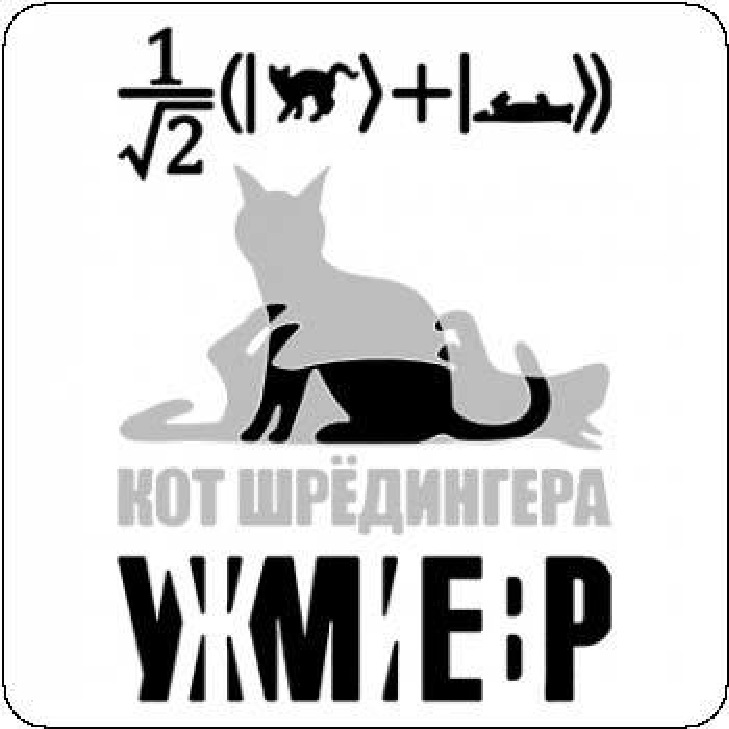
\includegraphics[scale=0.45]{sc.pdf}
\end{center}

}

\frame{

\frametitle{Операторы}
% TODO Операторы
}

\frame{

\frametitle{Запутаность}
% TODO Запутаность
}



\frame{

\frametitle{Квантовые потоки}
% TODO Квантовые потоки
}
\frame{

\frametitle{Квантовые потоки}

}
\frame{

\frametitle{Квантовые потоки}

}
\frame{

\frametitle{Квантовые потоки}

}


\frame{

\frametitle{Квантовое лямбда-исчисление}
% TODO Квантовое лямбда-исчисление
}

% % % % % % % % % % % % % % 

\frame{

\frametitle{Джозефсоновские кубиты}
\begin{center}
 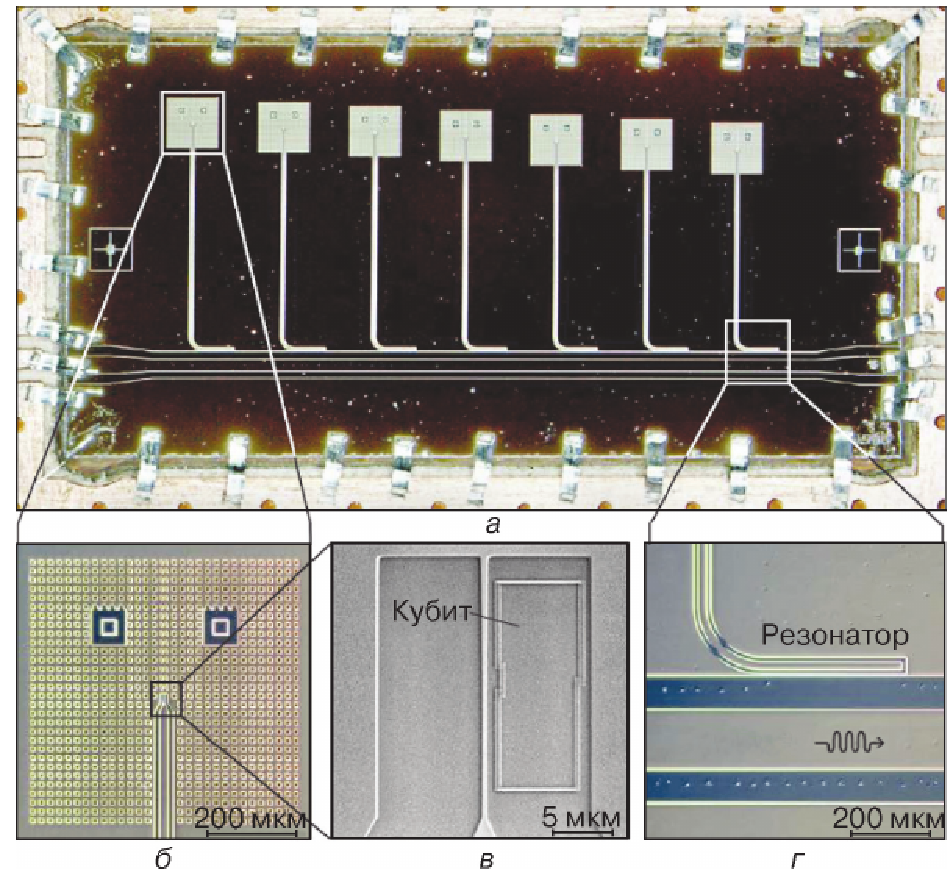
\includegraphics[scale=0.4]{q_jj.pdf}

\end{center}
\tiny M. Jerger, S. Poletto, P. Macha, U. Hübner, A. Lukashenko, E. Il’ichev, A. V. Ustinov \textit{Readout of a qubit array via a single transmission line}, Europhys. Lett. 96, (2011) 40012
}


\frame{

\frametitle{Джозефсоновские кубиты}
% TODO Джозефсоновские кубиты

\begin{center}
\begin{tabular}{cc}
 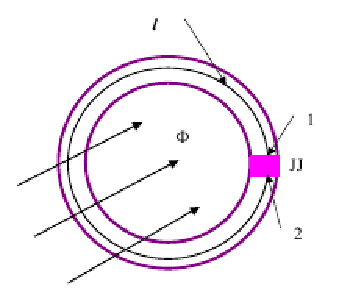
\includegraphics[scale=0.6]{jj.pdf} &
 
\end{tabular}


\end{center}
}

\frame{

\frametitle{D-Wave}
\begin{center}
 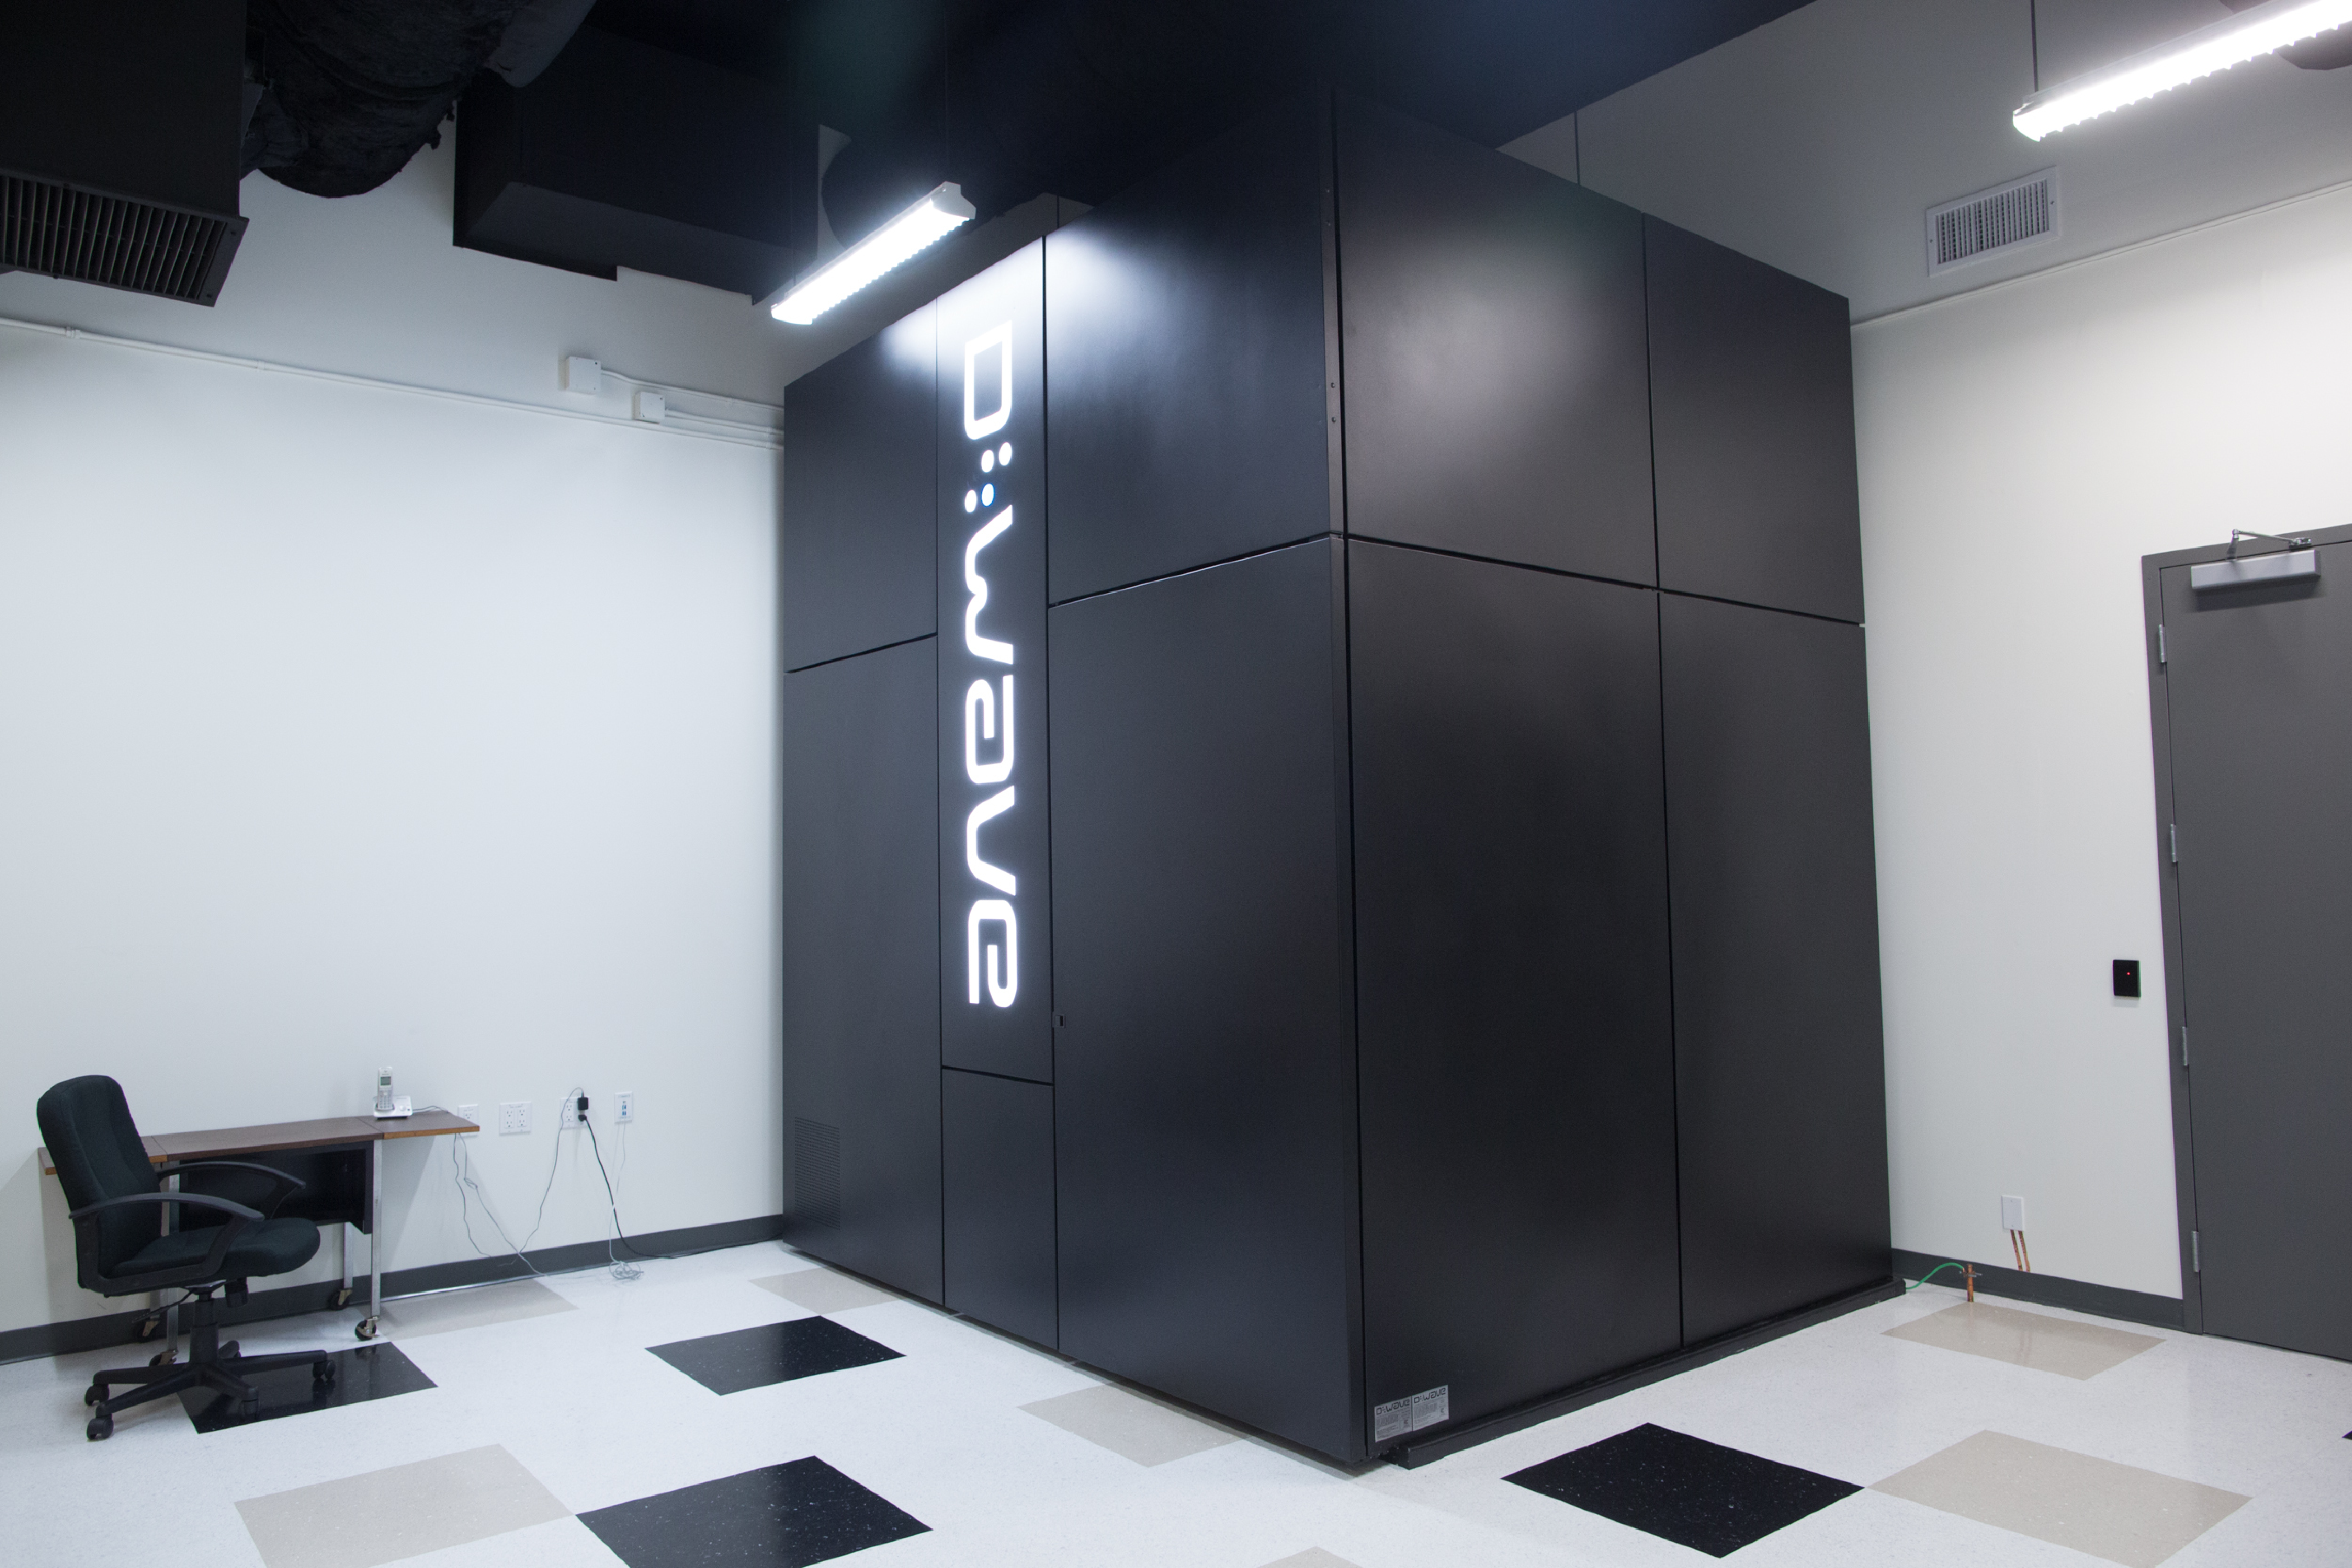
\includegraphics[scale=0.1]{dw.pdf}
 
\tiny
Sergio Boixo, Troels F. Rønnow, Sergei V. Isakov, Zhihui Wang, David Wecker, Daniel A. Lidar, John M. Martinis, Matthias Troyer  \textit{Quantum annealing with more than one hundred qubits},  	arXiv:1304.4595 
\end{center}
}

% % % % % % % % % % % % % % 

\frame{

\frametitle{Универсальная задача перебора}
% TODO Универсальная задача перебора

}

\frame{

\frametitle{Оптимальность алгоритма Гровера...}

}


\frame{

\frametitle{Оптимальность алгоритма Гровера... или почему $\mathcal{P}\neq\mathcal{NP} $}
\begin{enumerate}
 \item Линейность\footnote{В смысле линейность \textbf{интегрального оператора}, а не подинтегрального выражения!} квантовой механики $\rightarrow$ Предел Гровера $\sqrt{N}$
\item А если у нас будут нелинейные квантовые операторы, сохраняющие нормировку? (``Приличная'' нелинейная КМ)
\end{enumerate}
}



\frame{
\frametitle{Оптимальность алгоритма Гровера... или почему $\mathcal{P}\neq\mathcal{NP} $}
\begin{enumerate}
 \item Линейность квантовой механики $\rightarrow$ Предел Гровера $\sqrt{N}$
\item Нелинейная КМ передает сигналы быстрее с и  решает $\mathcal{\#P}$-полные проблемы за полиномиальное время!\footnote{Ограничиваясь нелинейными преобразованиями \textbf{сохраняющими норму}} Ура!
\end{enumerate}
}

\frame{
\frametitle{Оптимальность алгоритма Гровера... или почему $\mathcal{P}\neq\mathcal{NP} $}
\begin{enumerate}
 \item Линейность квантовой механики $\rightarrow$ Предел Гровера $\sqrt{N}$
\item Нелинейная КМ передает сигналы быстрее с и  решает $\mathcal{\#P}$-полные проблемы за полиномиальное время! Ура!
\item ... попутно экспоненциально размножая ошибку. \#\$\^\%\&*!
\end{enumerate}
}

\frame{
\frametitle{Оптимальность алгоритма Гровера... или почему $\mathcal{P}\neq\mathcal{NP} $}
\begin{enumerate}
 \item Линейность квантовой механики $\rightarrow$ Предел Гровера $\sqrt{N}$
\item Нелинейная КМ передает сигналы быстрее с и  решает $\mathcal{\#P}$-полные проблемы за полиномиальное время! Ура!
\item ... попутно экспоненциально размножая ошибку. \#\$\^\%\&*!
\item Скрытые параметры? Предел Гровера улучшается с $N^\frac{1}{2}$ до $N^\frac{1}{3}$ -- поиск по ``историям'' траекторий частичек
\end{enumerate}
}

\frame{
\frametitle{Оптимальность алгоритма Гровера... или почему $\mathcal{P}\neq\mathcal{NP} $}
\begin{enumerate}
 \item Линейность квантовой механики $\rightarrow$ Предел Гровера $\sqrt{N}$
\item Нелинейная КМ передает сигналы быстрее с и  решает $\mathcal{\#P}$-полные проблемы за полиномиальное время! Ура!
\item ... попутно экспоненциально размножая ошибку. \#\$\^\%\&*!
\item Скрытые параметры? Предел Гровера улучшается с $N^\frac{1}{2}$ до $N^\frac{1}{3}$ -- поиск по ``историям'' траекторий частичек
\item Зеноновские вычисления и всякие прочие супертьюринговые вычисления  накрываются по достижении планковской длины.  
\end{enumerate}
}


\frame{

\frametitle{Алгоритм Шора}
% TODO Алгоритм Шора

}

\frame{

\frametitle{Алгоритм Шора}

}

% % % % % % % % % % % % % % 

\frame{

\frametitle{Симметричные и ассиметричные криптосистемы}
% TODO Симметричные и ассиметричные криптосистемы
}


\frame{

\frametitle{Задача о скрытой подгруппе}
% TODO Задача о скрытой подгруппе

}

\frame{

\frametitle{Неабелевый случай}
% TODO Неабелевый случай

}

% % % % % % % % % % % % % % 

\frame{

\frametitle{Влияние -- квантовая связь}
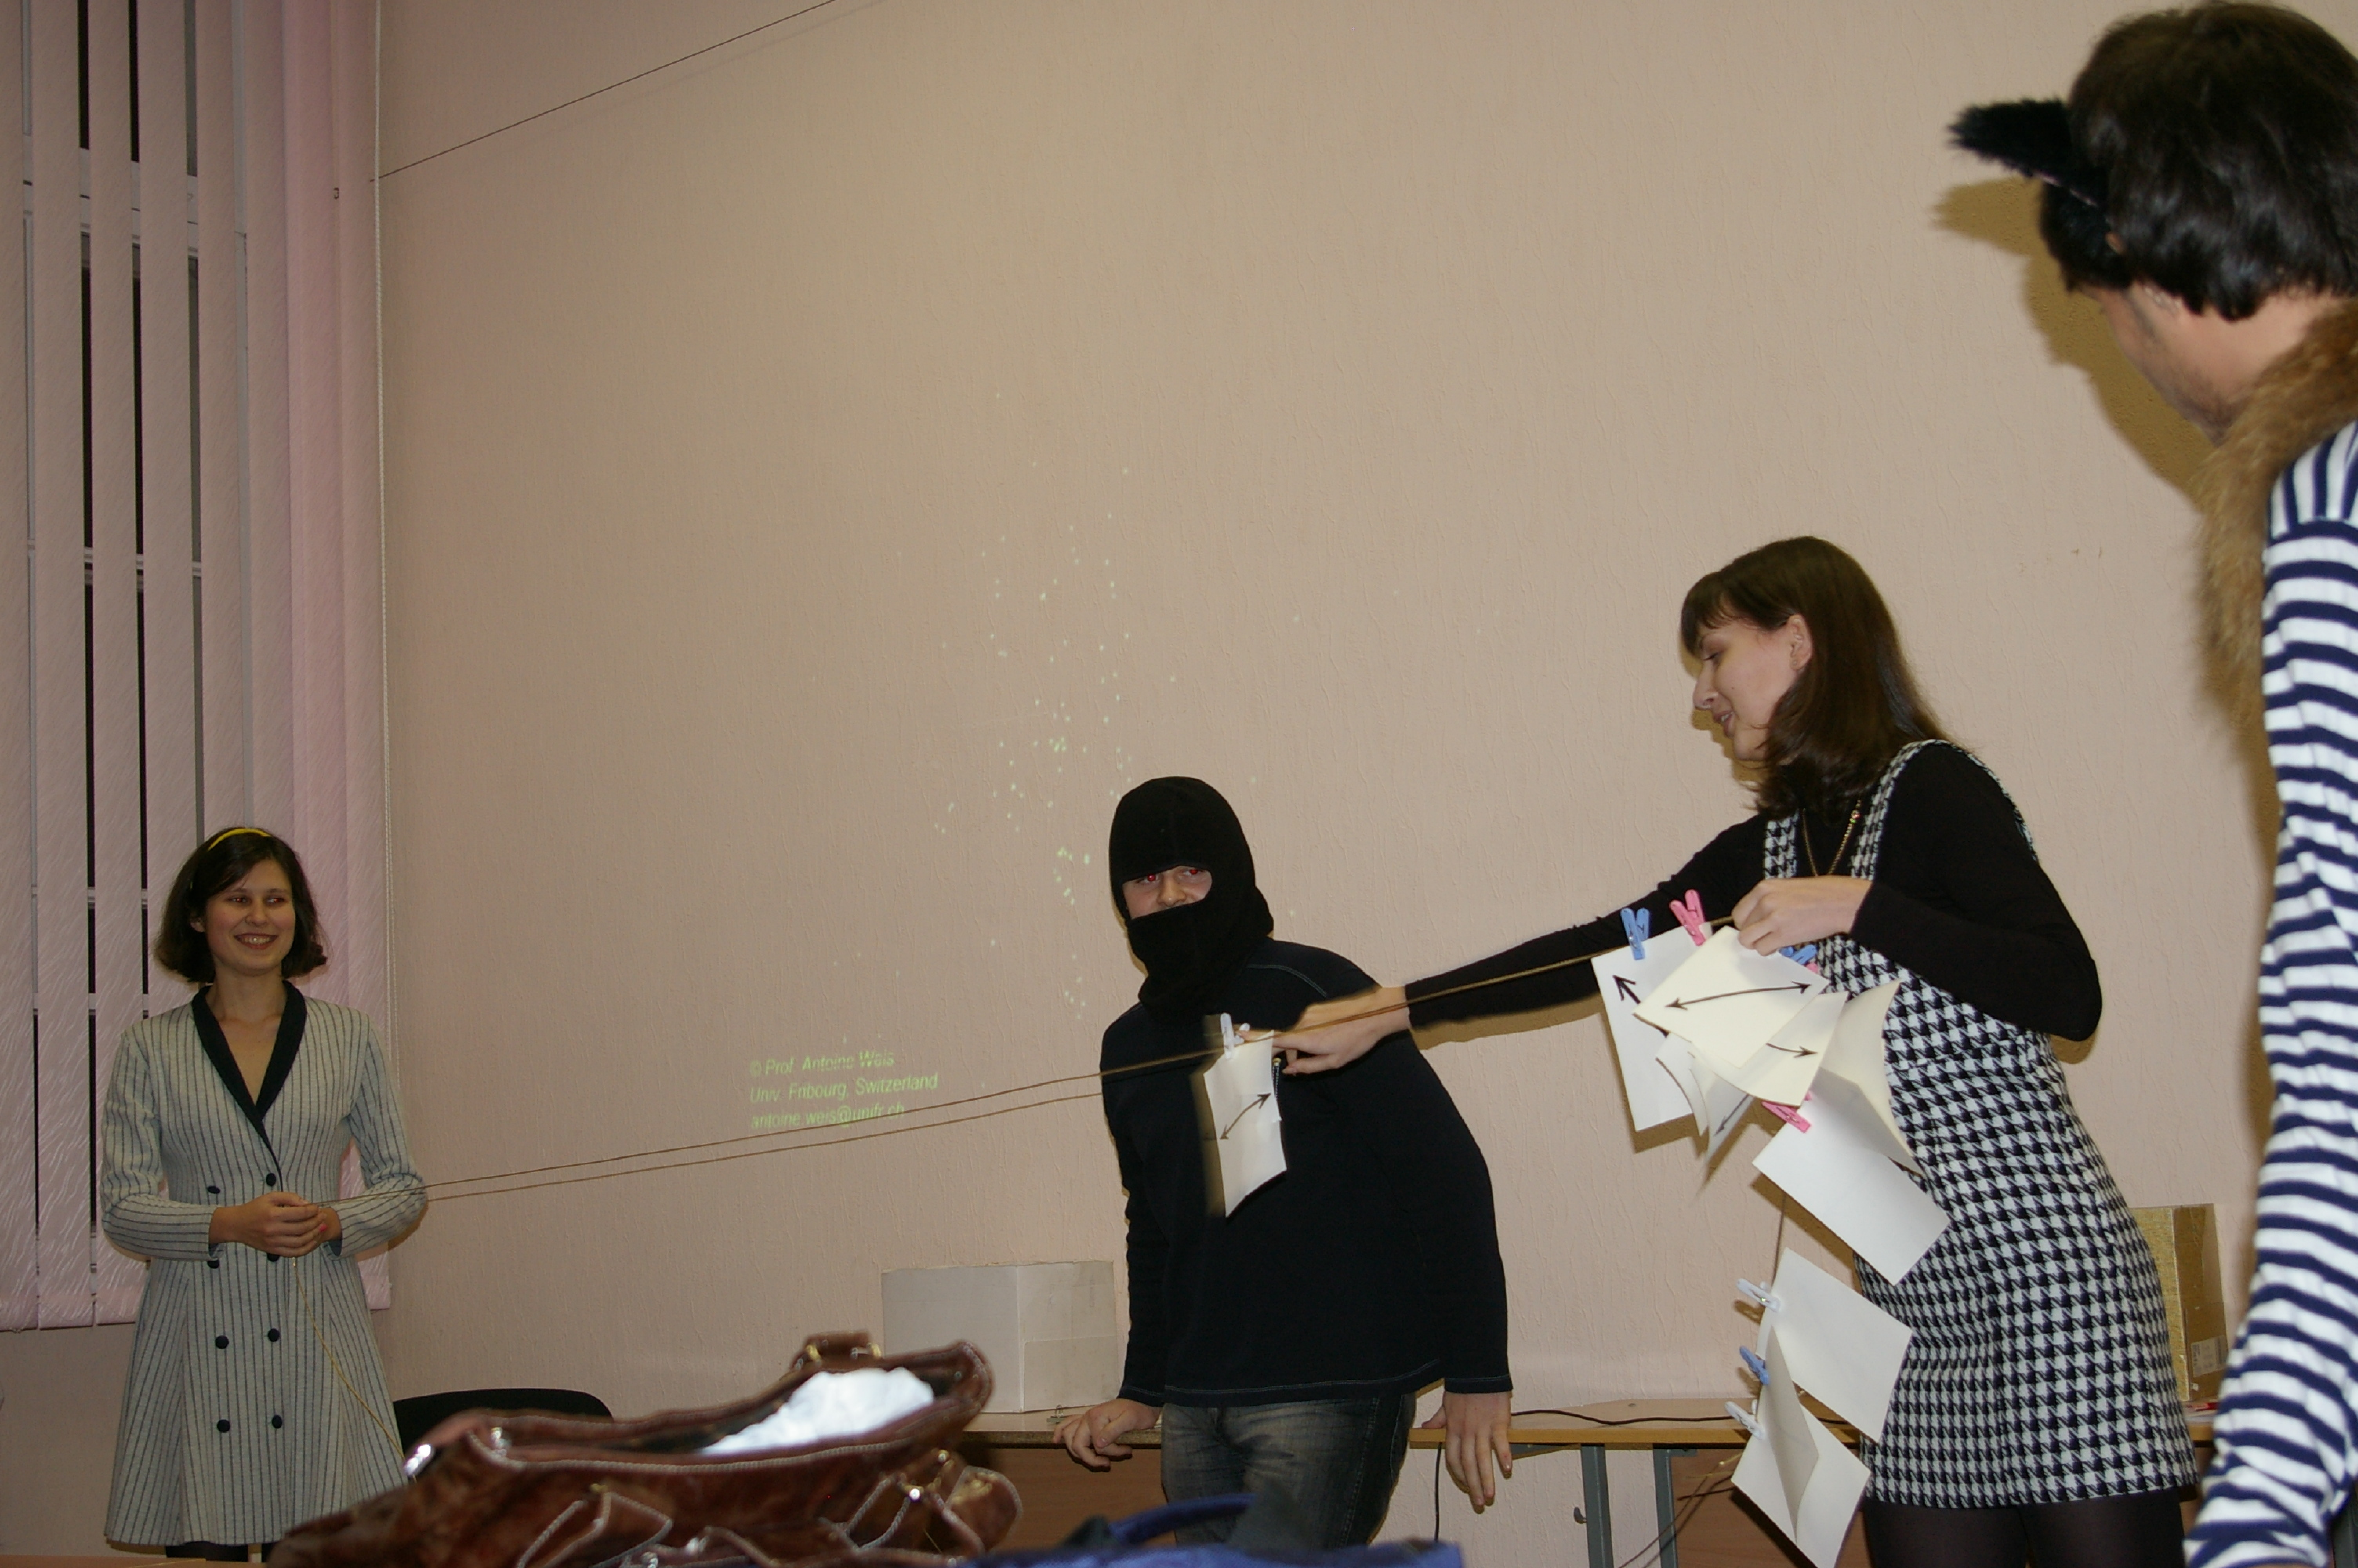
\includegraphics[scale=0.1]{qp1.pdf}
}

\frame{

\frametitle{Влияние -- квантовая связь}
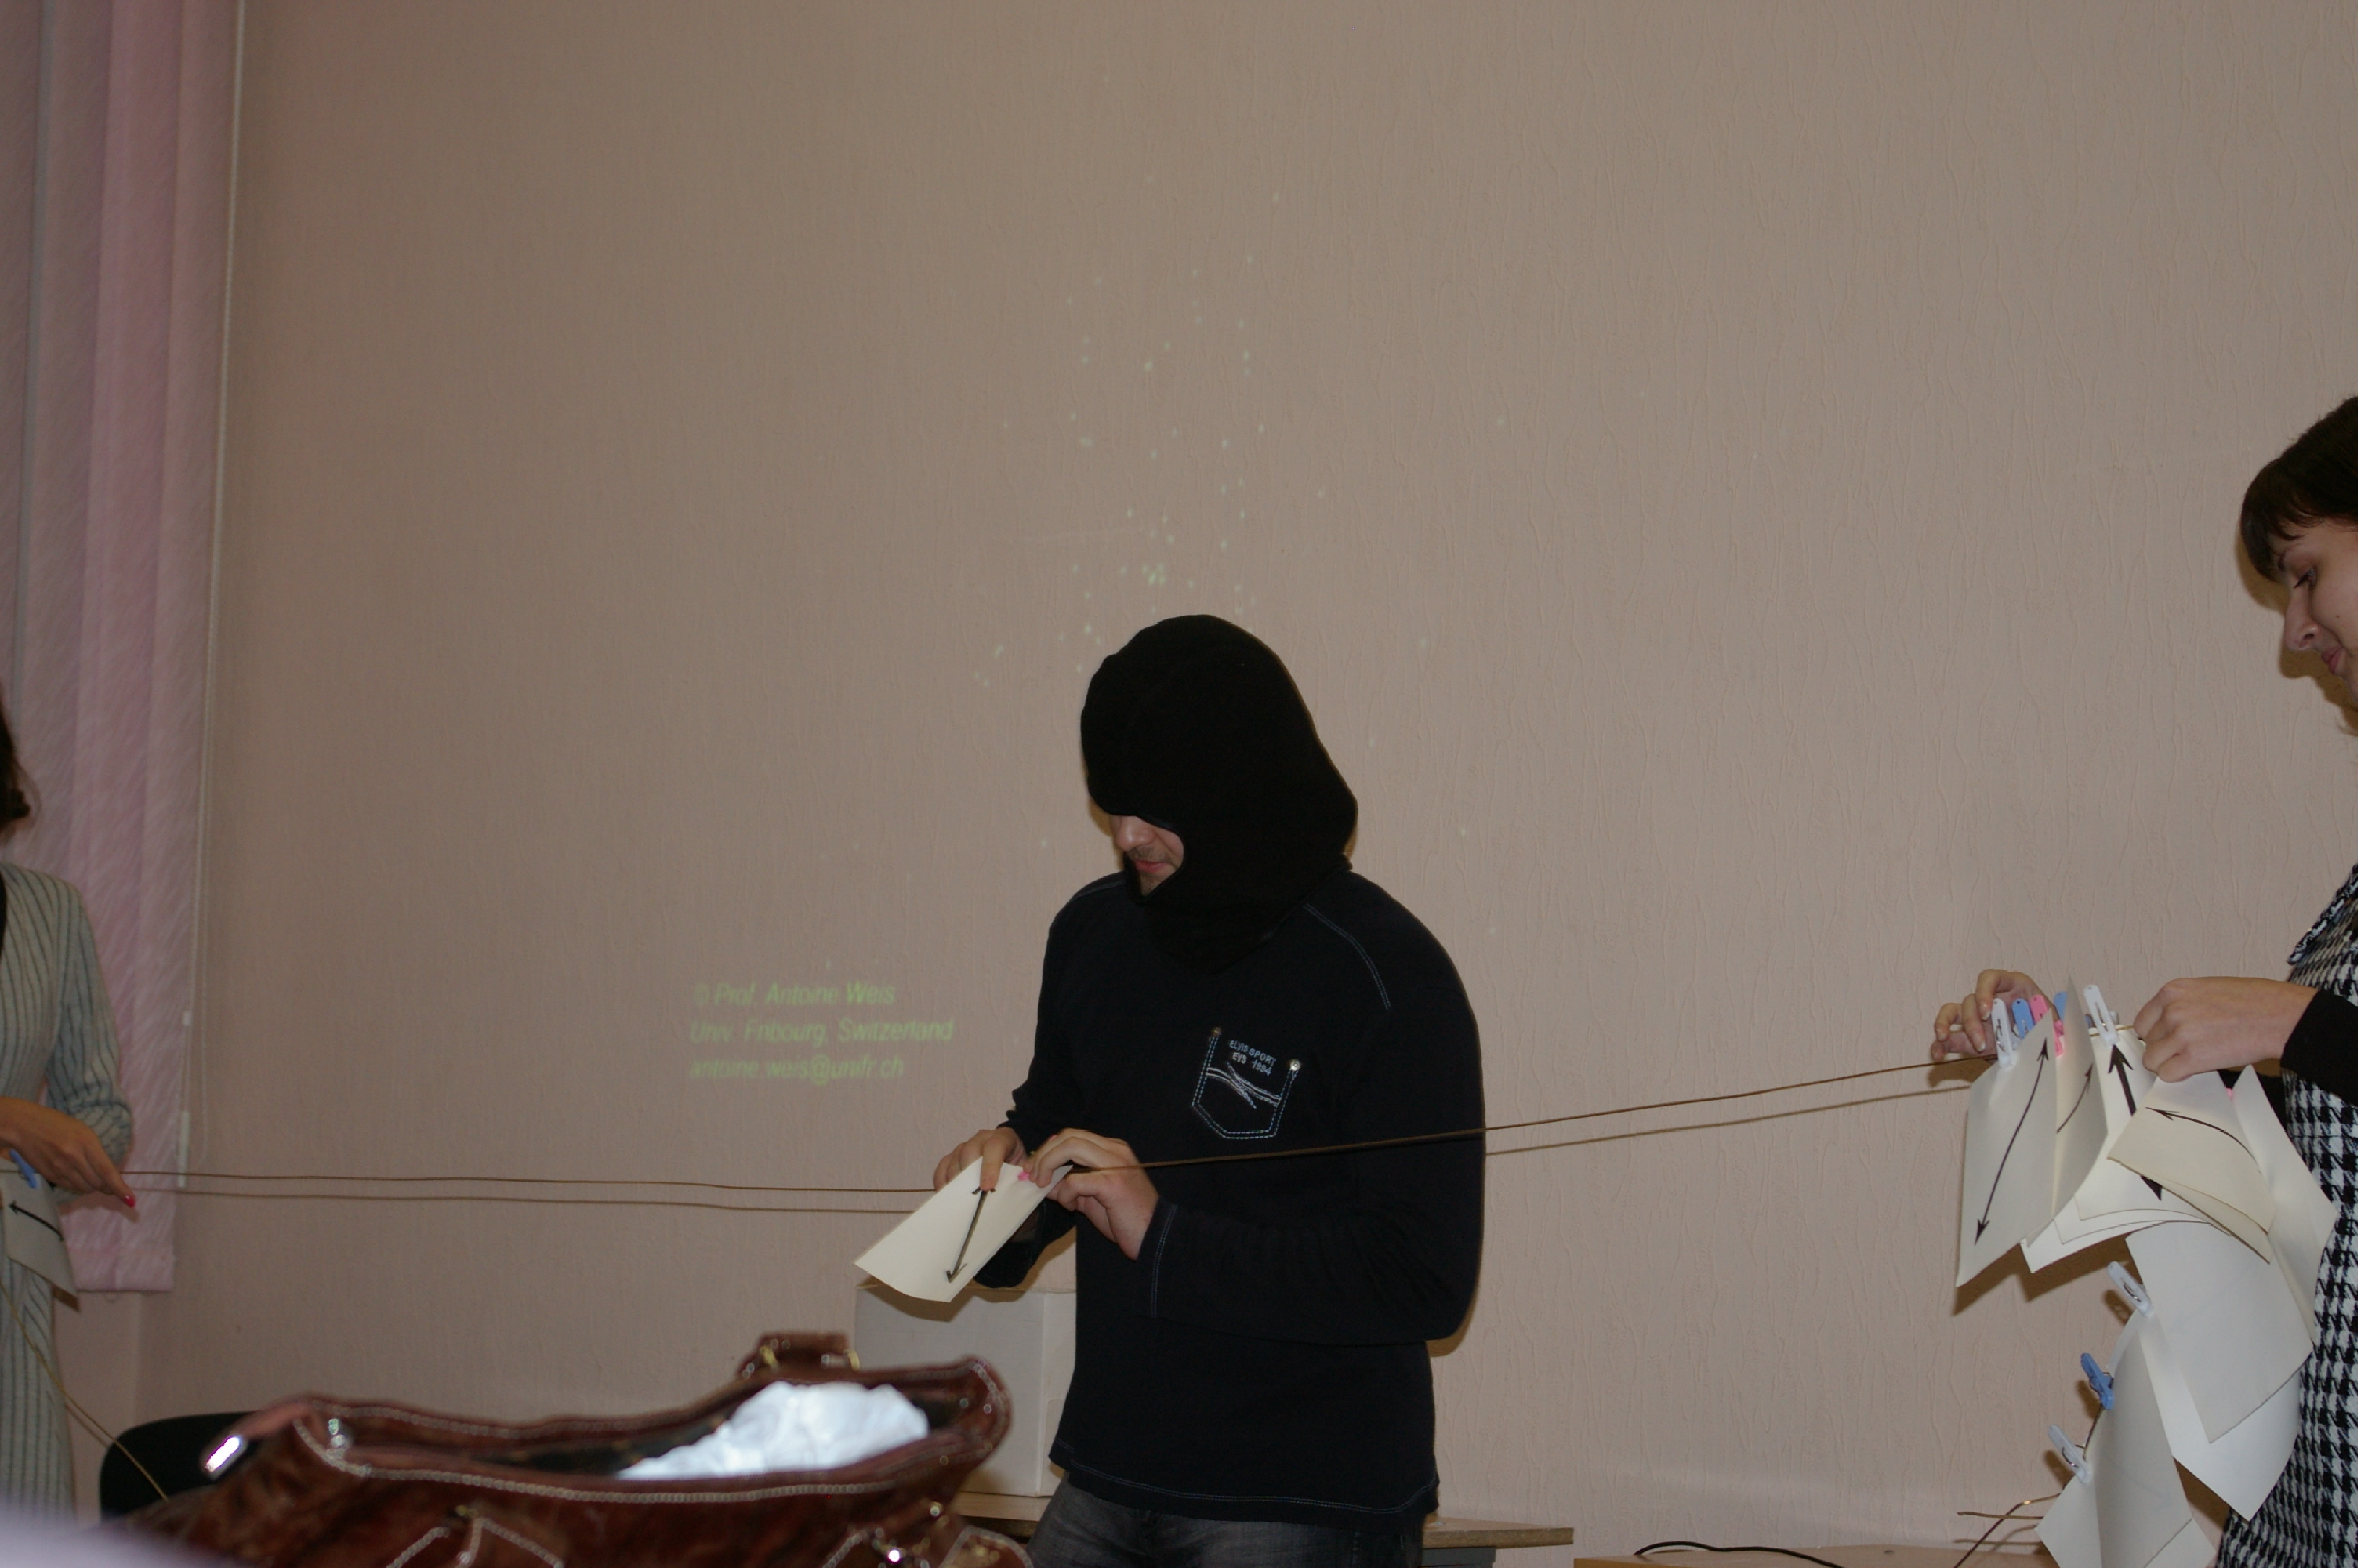
\includegraphics[scale=0.1]{qp2.pdf}
}

\frame{

\frametitle{Влияние -- цифровая физика}
Широко известные не в столь узких кругах обсуждения ``информационных'' аспектов физики:
\begin{itemize}
 \item Konrad Zuse \textit{Rechnender Raum}\footnote{Вычислительное пространство} (1967)
\item Lloyd, S., \textit{Programming the Universe: A Quantum Computer Scientist Takes On the Cosmos} (2006)
\item Хокинг, Прескилл,Сасскинд  и срачик о термодинамике черных дыр, которые ``теряют'' информацию.

\end{itemize}

}

\frame{
\frametitle{Влияние -- цифровая физика}
Интерпретации квантовой механики:
\begin{enumerate}
 \item Копенгагенская
\item Многомировая
\item Теории скрытого параметра(Schrödinger, Bohmian Mechanics )
\end{enumerate}
\begin{center}
\large В чем же разница? 
\end{center}

}

\frame{
\frametitle{Влияние -- цифровая физика}
Интерпретации квантовой механики:
\begin{enumerate}
 \item Копенгагенская
\item Многомировая
\item Теории скрытого параметра(Schrödinger, Bohmian Mechanics )
\end{enumerate}
\begin{center}
\large В чем же разница? 



\Huge РАЗНЫЕ ВСЕЛЕННЫЕ!

\normalsize
с разными вычислительными ресурсами!
\end{center}


}

\frame{

\frametitle{Влияние -- матан}
% TODO матан
\begin{astat}
   We should expect a mathematical question to have a definite answer, if and only if we can phrase
the question in terms of a physical process we can imagine.
\end{astat}



David Deutsch



У нас есть разные модели для 
}

% \frame{
% 
% \frametitle{Влияние -- теория эволюции}
% 
% }


\frame{

\frametitle{Влияние -- теория сознания}
% TODO теория сознания

}

\frame{

\frametitle{Аналитическая машина}
\begin{center}
 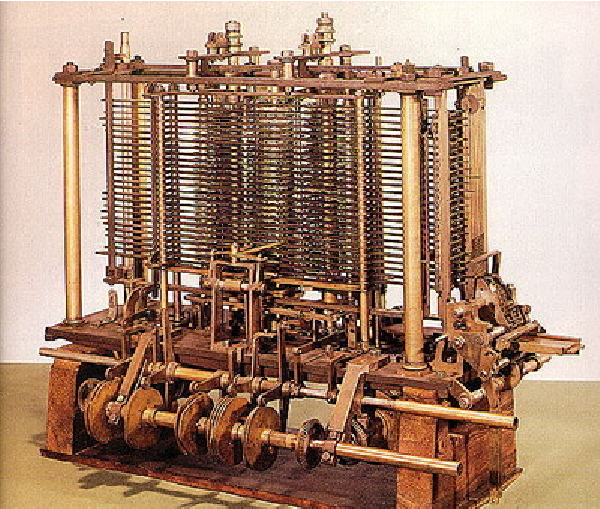
\includegraphics[scale=0.8]{de.pdf}

\end{center}

}



% % % % % % % % % % % % % % 

\frame{

\frametitle{Квантовое Функциональное Программирование}
% TODO Квантовое Функциональное Программирование
}
\frame{

\frametitle{Квантовое Функциональное Программирование}

}
\frame{

\frametitle{Квантовое Функциональное Программирование}

}


\frame{

\frametitle{Scheme simulator}
\begin{description}
  \item[Что?] Scheme
 \item[Где?] http://www.het.brown.edu/people/andre/qlambda/
 \item[Кто виноват?] André van Tonder.
\end{description}
}

% \frame{
% 
% \frametitle{Scheme simulator}
% 
% }
% 
% \frame{
% 
% \frametitle{Scheme simulator}
% 
% }

\frame{

\frametitle{QIO -- Quantum IO Monad }
\begin{description}
  \item[Что?] Haskell
 \item[Где?] http://hackage.haskell.org/package/QIO
 \item[Кто виноват?] Alexander S. Green
\end{description}

}

% \frame{
% 
% \frametitle{QIO -- Quantum IO Monad }
% 
% }
% 
% \frame{
% 
% \frametitle{QIO -- Quantum IO Monad }
% 
% }

\frame{

\frametitle{Maxima -- qinf}
\begin{description}
  \item[Что?] Maxima
 \item[Где?] http://www.johnlapeyre.com/qinf/
 \item[Кто виноват?] G. John Lapeyre, Jr.
\end{description}
}

\frame{
\frametitle{List of QC simulators}
\begin{itemize}
 \item http://www.quantiki.org/wiki/List\_of\_QC\_simulators
 \item curl, grep, sort -u, wc -l, немного магии...
 \item 95
 \item ??????
 \item PROFIT
\end{itemize}

}







% % % % % % % % % % % % % % 
\frame{

\frametitle{Что почитать?}
Книги/лекции:
\begin{itemize}
 \item \textbf{CS191x} Quantum Mechanics and Quantum Computation
 \item \textbf{Лекции} -- Preskill(Caltech), Vazirani(Berkeley), Watrous(Waterloo), ...
 \item \textbf{Reference textbook} -- Nielsen and Chuang, \textit{Quantum Computation and Quantum Information}\footnote{Нильсен М., Чанг И. \textit{Квантовые вычисления и квантовая информация}. Пер. с англ - М.: Мир, 2006. - 824с}
 \item А. Китаев, А. Шень, М. Вялый. \textit{Классические и квантовые вычисления.}
 \item MIT OCW 6.845 \textit{Quantum Complexity Theory} -- Scott Aaronson
 \item Scott Aaronson \textit{Quantum Computing Since Democritus}
 \item Feynman lectures on computation

\end{itemize}


}

\frame{
\frametitle{Что почитать?}
Статьи:
\begin{itemize}
 \item Feynman, R. P. (1982). \textit{"Simulating physics with computers"}. (Перепечетано в Feynman lectures on computation)
 \item \textit{Quantum annealing with more than one hundred qubits},  	arXiv:1304.4595 
 \item \textit{Physics, Topology, Logic and Computation: A Rosetta Stone},  	arXiv:0903.0340
 \item \textit{Quantum Proofs for Classical Theorems}, 10.4086/toc.gs.2011.002
 \item \textit{NP-complete Problems and Physical Reality},  quant-ph/0502072

\end{itemize}


}
% % % % % % % % % % % % % % 

\frame{

\begin{center}
 \frametitle{Feci, quod potui, faciant meliora potentes}
\Huge Dixi\end{center}
}



%%%%%%%%%%%%%%%%%%%%%%%%%%%%%%%%%%%%%%%%%%%%%%%%%%%

% \frame{
% \frametitle{}
% 
% \begin{figure}[ht]
%  \includemovie[
%  poster,
%  text={\small P vs NP}
% ]{0.5\linewidth}{0.5\linewidth}{pnp.mp4}
% \end{figure}
% }

\end{document}
